% Created by tikzDevice version 0.12 on 2019-03-22 17:26:06
% !TEX encoding = UTF-8 Unicode
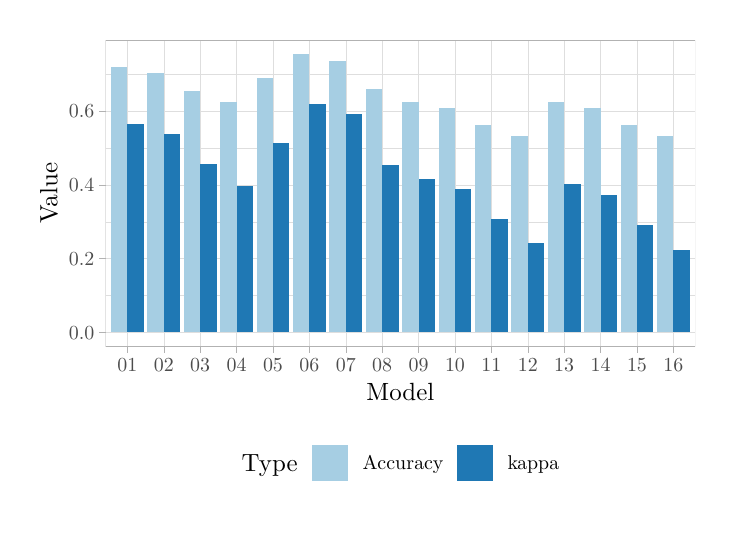
\begin{tikzpicture}[x=1pt,y=1pt]
\definecolor{fillColor}{RGB}{255,255,255}
\path[use as bounding box,fill=fillColor,fill opacity=0.00] (0,0) rectangle (245.72,173.45);
\begin{scope}
\path[clip] (  0.00,  0.00) rectangle (245.72,173.45);
\definecolor{drawColor}{RGB}{255,255,255}
\definecolor{fillColor}{RGB}{255,255,255}

\path[draw=drawColor,line width= 0.5pt,line join=round,line cap=round,fill=fillColor] (  0.00,  0.00) rectangle (245.72,173.45);
\end{scope}
\begin{scope}
\path[clip] ( 28.14, 58.30) rectangle (241.22,168.95);
\definecolor{fillColor}{RGB}{255,255,255}

\path[fill=fillColor] ( 28.14, 58.30) rectangle (241.22,168.95);
\definecolor{drawColor}{gray}{0.87}

\path[draw=drawColor,line width= 0.1pt,line join=round] ( 28.14, 76.66) --
	(241.22, 76.66);

\path[draw=drawColor,line width= 0.1pt,line join=round] ( 28.14,103.33) --
	(241.22,103.33);

\path[draw=drawColor,line width= 0.1pt,line join=round] ( 28.14,130.00) --
	(241.22,130.00);

\path[draw=drawColor,line width= 0.1pt,line join=round] ( 28.14,156.67) --
	(241.22,156.67);

\path[draw=drawColor,line width= 0.2pt,line join=round] ( 28.14, 63.33) --
	(241.22, 63.33);

\path[draw=drawColor,line width= 0.2pt,line join=round] ( 28.14, 90.00) --
	(241.22, 90.00);

\path[draw=drawColor,line width= 0.2pt,line join=round] ( 28.14,116.66) --
	(241.22,116.66);

\path[draw=drawColor,line width= 0.2pt,line join=round] ( 28.14,143.33) --
	(241.22,143.33);

\path[draw=drawColor,line width= 0.2pt,line join=round] ( 36.03, 58.30) --
	( 36.03,168.95);

\path[draw=drawColor,line width= 0.2pt,line join=round] ( 49.18, 58.30) --
	( 49.18,168.95);

\path[draw=drawColor,line width= 0.2pt,line join=round] ( 62.34, 58.30) --
	( 62.34,168.95);

\path[draw=drawColor,line width= 0.2pt,line join=round] ( 75.49, 58.30) --
	( 75.49,168.95);

\path[draw=drawColor,line width= 0.2pt,line join=round] ( 88.64, 58.30) --
	( 88.64,168.95);

\path[draw=drawColor,line width= 0.2pt,line join=round] (101.80, 58.30) --
	(101.80,168.95);

\path[draw=drawColor,line width= 0.2pt,line join=round] (114.95, 58.30) --
	(114.95,168.95);

\path[draw=drawColor,line width= 0.2pt,line join=round] (128.10, 58.30) --
	(128.10,168.95);

\path[draw=drawColor,line width= 0.2pt,line join=round] (141.26, 58.30) --
	(141.26,168.95);

\path[draw=drawColor,line width= 0.2pt,line join=round] (154.41, 58.30) --
	(154.41,168.95);

\path[draw=drawColor,line width= 0.2pt,line join=round] (167.56, 58.30) --
	(167.56,168.95);

\path[draw=drawColor,line width= 0.2pt,line join=round] (180.71, 58.30) --
	(180.71,168.95);

\path[draw=drawColor,line width= 0.2pt,line join=round] (193.87, 58.30) --
	(193.87,168.95);

\path[draw=drawColor,line width= 0.2pt,line join=round] (207.02, 58.30) --
	(207.02,168.95);

\path[draw=drawColor,line width= 0.2pt,line join=round] (220.17, 58.30) --
	(220.17,168.95);

\path[draw=drawColor,line width= 0.2pt,line join=round] (233.33, 58.30) --
	(233.33,168.95);
\definecolor{fillColor}{RGB}{31,120,180}

\path[fill=fillColor] ( 36.03, 63.33) rectangle ( 41.95,138.65);
\definecolor{fillColor}{RGB}{166,206,227}

\path[fill=fillColor] ( 30.11, 63.33) rectangle ( 36.03,159.24);
\definecolor{fillColor}{RGB}{31,120,180}

\path[fill=fillColor] ( 49.18, 63.33) rectangle ( 55.10,134.88);
\definecolor{fillColor}{RGB}{166,206,227}

\path[fill=fillColor] ( 43.27, 63.33) rectangle ( 49.18,156.90);
\definecolor{fillColor}{RGB}{31,120,180}

\path[fill=fillColor] ( 62.34, 63.33) rectangle ( 68.26,124.31);
\definecolor{fillColor}{RGB}{166,206,227}

\path[fill=fillColor] ( 56.42, 63.33) rectangle ( 62.34,150.66);
\definecolor{fillColor}{RGB}{31,120,180}

\path[fill=fillColor] ( 75.49, 63.33) rectangle ( 81.41,116.37);
\definecolor{fillColor}{RGB}{166,206,227}

\path[fill=fillColor] ( 69.57, 63.33) rectangle ( 75.49,146.76);
\definecolor{fillColor}{RGB}{31,120,180}

\path[fill=fillColor] ( 88.64, 63.33) rectangle ( 94.56,131.68);
\definecolor{fillColor}{RGB}{166,206,227}

\path[fill=fillColor] ( 82.72, 63.33) rectangle ( 88.64,155.34);
\definecolor{fillColor}{RGB}{31,120,180}

\path[fill=fillColor] (101.80, 63.33) rectangle (107.72,145.91);
\definecolor{fillColor}{RGB}{166,206,227}

\path[fill=fillColor] ( 95.88, 63.33) rectangle (101.80,163.92);
\definecolor{fillColor}{RGB}{31,120,180}

\path[fill=fillColor] (114.95, 63.33) rectangle (120.87,142.16);
\definecolor{fillColor}{RGB}{166,206,227}

\path[fill=fillColor] (109.03, 63.33) rectangle (114.95,161.58);
\definecolor{fillColor}{RGB}{31,120,180}

\path[fill=fillColor] (128.10, 63.33) rectangle (134.02,123.91);
\definecolor{fillColor}{RGB}{166,206,227}

\path[fill=fillColor] (122.18, 63.33) rectangle (128.10,151.44);
\definecolor{fillColor}{RGB}{31,120,180}

\path[fill=fillColor] (141.26, 63.33) rectangle (147.17,118.94);
\definecolor{fillColor}{RGB}{166,206,227}

\path[fill=fillColor] (135.34, 63.33) rectangle (141.26,146.76);
\definecolor{fillColor}{RGB}{31,120,180}

\path[fill=fillColor] (154.41, 63.33) rectangle (160.33,115.10);
\definecolor{fillColor}{RGB}{166,206,227}

\path[fill=fillColor] (148.49, 63.33) rectangle (154.41,144.42);
\definecolor{fillColor}{RGB}{31,120,180}

\path[fill=fillColor] (167.56, 63.33) rectangle (173.48,104.24);
\definecolor{fillColor}{RGB}{166,206,227}

\path[fill=fillColor] (161.64, 63.33) rectangle (167.56,138.19);
\definecolor{fillColor}{RGB}{31,120,180}

\path[fill=fillColor] (180.71, 63.33) rectangle (186.63, 95.80);
\definecolor{fillColor}{RGB}{166,206,227}

\path[fill=fillColor] (174.80, 63.33) rectangle (180.71,134.29);
\definecolor{fillColor}{RGB}{31,120,180}

\path[fill=fillColor] (193.87, 63.33) rectangle (199.79,117.07);
\definecolor{fillColor}{RGB}{166,206,227}

\path[fill=fillColor] (187.95, 63.33) rectangle (193.87,146.76);
\definecolor{fillColor}{RGB}{31,120,180}

\path[fill=fillColor] (207.02, 63.33) rectangle (212.94,113.13);
\definecolor{fillColor}{RGB}{166,206,227}

\path[fill=fillColor] (201.10, 63.33) rectangle (207.02,144.42);
\definecolor{fillColor}{RGB}{31,120,180}

\path[fill=fillColor] (220.17, 63.33) rectangle (226.09,101.98);
\definecolor{fillColor}{RGB}{166,206,227}

\path[fill=fillColor] (214.25, 63.33) rectangle (220.17,138.19);
\definecolor{fillColor}{RGB}{31,120,180}

\path[fill=fillColor] (233.33, 63.33) rectangle (239.25, 93.28);
\definecolor{fillColor}{RGB}{166,206,227}

\path[fill=fillColor] (227.41, 63.33) rectangle (233.33,134.29);
\definecolor{drawColor}{gray}{0.70}

\path[draw=drawColor,line width= 0.5pt,line join=round,line cap=round] ( 28.14, 58.30) rectangle (241.22,168.95);
\end{scope}
\begin{scope}
\path[clip] (  0.00,  0.00) rectangle (245.72,173.45);
\definecolor{drawColor}{gray}{0.30}

\node[text=drawColor,anchor=base east,inner sep=0pt, outer sep=0pt, scale=  0.72] at ( 24.09, 60.85) {0.0};

\node[text=drawColor,anchor=base east,inner sep=0pt, outer sep=0pt, scale=  0.72] at ( 24.09, 87.52) {0.2};

\node[text=drawColor,anchor=base east,inner sep=0pt, outer sep=0pt, scale=  0.72] at ( 24.09,114.19) {0.4};

\node[text=drawColor,anchor=base east,inner sep=0pt, outer sep=0pt, scale=  0.72] at ( 24.09,140.85) {0.6};
\end{scope}
\begin{scope}
\path[clip] (  0.00,  0.00) rectangle (245.72,173.45);
\definecolor{drawColor}{gray}{0.70}

\path[draw=drawColor,line width= 0.2pt,line join=round] ( 25.89, 63.33) --
	( 28.14, 63.33);

\path[draw=drawColor,line width= 0.2pt,line join=round] ( 25.89, 90.00) --
	( 28.14, 90.00);

\path[draw=drawColor,line width= 0.2pt,line join=round] ( 25.89,116.66) --
	( 28.14,116.66);

\path[draw=drawColor,line width= 0.2pt,line join=round] ( 25.89,143.33) --
	( 28.14,143.33);
\end{scope}
\begin{scope}
\path[clip] (  0.00,  0.00) rectangle (245.72,173.45);
\definecolor{drawColor}{gray}{0.70}

\path[draw=drawColor,line width= 0.2pt,line join=round] ( 36.03, 56.05) --
	( 36.03, 58.30);

\path[draw=drawColor,line width= 0.2pt,line join=round] ( 49.18, 56.05) --
	( 49.18, 58.30);

\path[draw=drawColor,line width= 0.2pt,line join=round] ( 62.34, 56.05) --
	( 62.34, 58.30);

\path[draw=drawColor,line width= 0.2pt,line join=round] ( 75.49, 56.05) --
	( 75.49, 58.30);

\path[draw=drawColor,line width= 0.2pt,line join=round] ( 88.64, 56.05) --
	( 88.64, 58.30);

\path[draw=drawColor,line width= 0.2pt,line join=round] (101.80, 56.05) --
	(101.80, 58.30);

\path[draw=drawColor,line width= 0.2pt,line join=round] (114.95, 56.05) --
	(114.95, 58.30);

\path[draw=drawColor,line width= 0.2pt,line join=round] (128.10, 56.05) --
	(128.10, 58.30);

\path[draw=drawColor,line width= 0.2pt,line join=round] (141.26, 56.05) --
	(141.26, 58.30);

\path[draw=drawColor,line width= 0.2pt,line join=round] (154.41, 56.05) --
	(154.41, 58.30);

\path[draw=drawColor,line width= 0.2pt,line join=round] (167.56, 56.05) --
	(167.56, 58.30);

\path[draw=drawColor,line width= 0.2pt,line join=round] (180.71, 56.05) --
	(180.71, 58.30);

\path[draw=drawColor,line width= 0.2pt,line join=round] (193.87, 56.05) --
	(193.87, 58.30);

\path[draw=drawColor,line width= 0.2pt,line join=round] (207.02, 56.05) --
	(207.02, 58.30);

\path[draw=drawColor,line width= 0.2pt,line join=round] (220.17, 56.05) --
	(220.17, 58.30);

\path[draw=drawColor,line width= 0.2pt,line join=round] (233.33, 56.05) --
	(233.33, 58.30);
\end{scope}
\begin{scope}
\path[clip] (  0.00,  0.00) rectangle (245.72,173.45);
\definecolor{drawColor}{gray}{0.30}

\node[text=drawColor,anchor=base,inner sep=0pt, outer sep=0pt, scale=  0.72] at ( 36.03, 49.29) {01};

\node[text=drawColor,anchor=base,inner sep=0pt, outer sep=0pt, scale=  0.72] at ( 49.18, 49.29) {02};

\node[text=drawColor,anchor=base,inner sep=0pt, outer sep=0pt, scale=  0.72] at ( 62.34, 49.29) {03};

\node[text=drawColor,anchor=base,inner sep=0pt, outer sep=0pt, scale=  0.72] at ( 75.49, 49.29) {04};

\node[text=drawColor,anchor=base,inner sep=0pt, outer sep=0pt, scale=  0.72] at ( 88.64, 49.29) {05};

\node[text=drawColor,anchor=base,inner sep=0pt, outer sep=0pt, scale=  0.72] at (101.80, 49.29) {06};

\node[text=drawColor,anchor=base,inner sep=0pt, outer sep=0pt, scale=  0.72] at (114.95, 49.29) {07};

\node[text=drawColor,anchor=base,inner sep=0pt, outer sep=0pt, scale=  0.72] at (128.10, 49.29) {08};

\node[text=drawColor,anchor=base,inner sep=0pt, outer sep=0pt, scale=  0.72] at (141.26, 49.29) {09};

\node[text=drawColor,anchor=base,inner sep=0pt, outer sep=0pt, scale=  0.72] at (154.41, 49.29) {10};

\node[text=drawColor,anchor=base,inner sep=0pt, outer sep=0pt, scale=  0.72] at (167.56, 49.29) {11};

\node[text=drawColor,anchor=base,inner sep=0pt, outer sep=0pt, scale=  0.72] at (180.71, 49.29) {12};

\node[text=drawColor,anchor=base,inner sep=0pt, outer sep=0pt, scale=  0.72] at (193.87, 49.29) {13};

\node[text=drawColor,anchor=base,inner sep=0pt, outer sep=0pt, scale=  0.72] at (207.02, 49.29) {14};

\node[text=drawColor,anchor=base,inner sep=0pt, outer sep=0pt, scale=  0.72] at (220.17, 49.29) {15};

\node[text=drawColor,anchor=base,inner sep=0pt, outer sep=0pt, scale=  0.72] at (233.33, 49.29) {16};
\end{scope}
\begin{scope}
\path[clip] (  0.00,  0.00) rectangle (245.72,173.45);
\definecolor{drawColor}{RGB}{0,0,0}

\node[text=drawColor,anchor=base,inner sep=0pt, outer sep=0pt, scale=  0.90] at (134.68, 38.90) {Model};
\end{scope}
\begin{scope}
\path[clip] (  0.00,  0.00) rectangle (245.72,173.45);
\definecolor{drawColor}{RGB}{0,0,0}

\node[text=drawColor,rotate= 90.00,anchor=base,inner sep=0pt, outer sep=0pt, scale=  0.90] at ( 10.70,113.62) {Value};
\end{scope}
\begin{scope}
\path[clip] (  0.00,  0.00) rectangle (245.72,173.45);
\definecolor{fillColor}{RGB}{255,255,255}

\path[fill=fillColor] ( 72.80,  4.50) rectangle (196.56, 27.95);
\end{scope}
\begin{scope}
\path[clip] (  0.00,  0.00) rectangle (245.72,173.45);
\definecolor{drawColor}{RGB}{0,0,0}

\node[text=drawColor,anchor=base west,inner sep=0pt, outer sep=0pt, scale=  0.90] at ( 77.30, 13.13) {Type};
\end{scope}
\begin{scope}
\path[clip] (  0.00,  0.00) rectangle (245.72,173.45);
\definecolor{fillColor}{RGB}{255,255,255}

\path[fill=fillColor] (102.04,  9.00) rectangle (116.50, 23.45);
\end{scope}
\begin{scope}
\path[clip] (  0.00,  0.00) rectangle (245.72,173.45);
\definecolor{fillColor}{RGB}{166,206,227}

\path[fill=fillColor] (102.75,  9.71) rectangle (115.79, 22.74);
\end{scope}
\begin{scope}
\path[clip] (  0.00,  0.00) rectangle (245.72,173.45);
\definecolor{fillColor}{RGB}{255,255,255}

\path[fill=fillColor] (154.51,  9.00) rectangle (168.96, 23.45);
\end{scope}
\begin{scope}
\path[clip] (  0.00,  0.00) rectangle (245.72,173.45);
\definecolor{fillColor}{RGB}{31,120,180}

\path[fill=fillColor] (155.22,  9.71) rectangle (168.25, 22.74);
\end{scope}
\begin{scope}
\path[clip] (  0.00,  0.00) rectangle (245.72,173.45);
\definecolor{drawColor}{RGB}{0,0,0}

\node[text=drawColor,anchor=base west,inner sep=0pt, outer sep=0pt, scale=  0.72] at (121.00, 13.75) {Accuracy};
\end{scope}
\begin{scope}
\path[clip] (  0.00,  0.00) rectangle (245.72,173.45);
\definecolor{drawColor}{RGB}{0,0,0}

\node[text=drawColor,anchor=base west,inner sep=0pt, outer sep=0pt, scale=  0.72] at (173.46, 13.75) {kappa};
\end{scope}
\end{tikzpicture}
